\chapter{Plano e execução de testes}\label{cap:testes}
\rubricaRobustez
\section{Procedimento geral e critério de avaliação}
Os testes foram realizados sobre o ESP32 real, EMQX Cloud, cliente MQTTX e assinante \texttt{gravador.py}. As evidências incluem screenshots da interface e do PowerShell, registros preservados em CSV, histórico de estados e diário manual. O critério adotado distingue \emph{resultado obtido} de comportamento esperado e não afirma medições que não foram instrumentadas, como corrente do rádio ou instante exato da queda elétrica do nó. O plano detalhado permanece no Apêndice~\ref{ap:testes}.
\begin{table}[H]\centering\caption{Casos de teste do ciclo 2 e resultados observados}\label{tab:testes}\scriptsize
\begin{tabular}{@{}L{.85cm}L{4.1cm}L{6.8cm}L{2cm}@{}}\toprule
Caso&Procedimento realizado&Resultado real / evidência&Situação\\\midrule
CT-01&Ler DHT11 e observar broker&Telemetria de \texttt{eq04-no02} exibida no MQTTX e escrita em CSV&\aprovado\\
CT-02&Publicar \texttt{periodo\_s=30} em \texttt{config}&Intervalo mudou de 5~s para aproximadamente 30~s; evidência no MQTTX&\aprovado\\
CT-03&Interromper Wi-Fi do ESP32 por cerca de 2 min&\texttt{offline} às 14h29min16s e \texttt{online} às 14h32min28s; backlog posterior&\aprovado\\
CT-04&Provocar queda não graciosa e inspecionar estado&Mensagens LWT \texttt{offline} observadas; tempo exato da detecção não medido&\parcial\\
CT-05&Pressionar EN e observar \texttt{boot\_id}&Transição 121 $\to$ 122, \texttt{seq} retorna a 1, sem falsa duplicação entre boots&\aprovado\\
CT-06&Interromper/reabrir o gravador com mesmo cliente&\texttt{session\_present} e recepção em lote de registros anteriores no retorno&\aprovado\\
CT-07&Observar início antes de NTP&Uma leitura \texttt{ts:null} registrada; horários válidos aparecem depois&\aprovado\\
CT-08&Analisar campanha com \texttt{qualidade.py}&3.082 telemetrias, 3.080 únicas, 0 lacunas internas, 2 duplicações&\aprovado\\
CT-09&Verificar TLS e controles do EMQX&Gravador valida TLS; ESP32 não valida CA sem configuração; ACL em modo blacklist&\parcial\\
CT-10&Instrumentar custo do rádio e autonomia&Não houve medição instrumental de corrente ou energia&\parcial\\\bottomrule\end{tabular}\fonte{Diário, logs MQTT, firmware e CSV da equipe eq04.}\end{table}
\section{Interrupção do Wi-Fi e retorno da fila}
Segundo o diário, a conectividade do nó foi interrompida às 14h29 de 23/10. O broker registrou \texttt{offline} às 14h29min16s e \texttt{online} às 14h32min28s: intervalo entre mensagens de estado de \textbf{192~s}. Isso não é, rigorosamente, o tempo de reconexão após o restabelecimento do Wi-Fi, pois o instante de reativação do roteador não foi cronometrado. Durante o retorno, o gravador recebeu mensagens antigas juntas; o pico final de \texttt{chegada-ts} de 217,544~s é compatível com backlog. \textbf{A ausência de saltos internos de \texttt{seq} é limitada aos itens efetivamente numerados}. A fila de 120 registros não foi testada em transbordamento.
\begin{figure}[H]\centering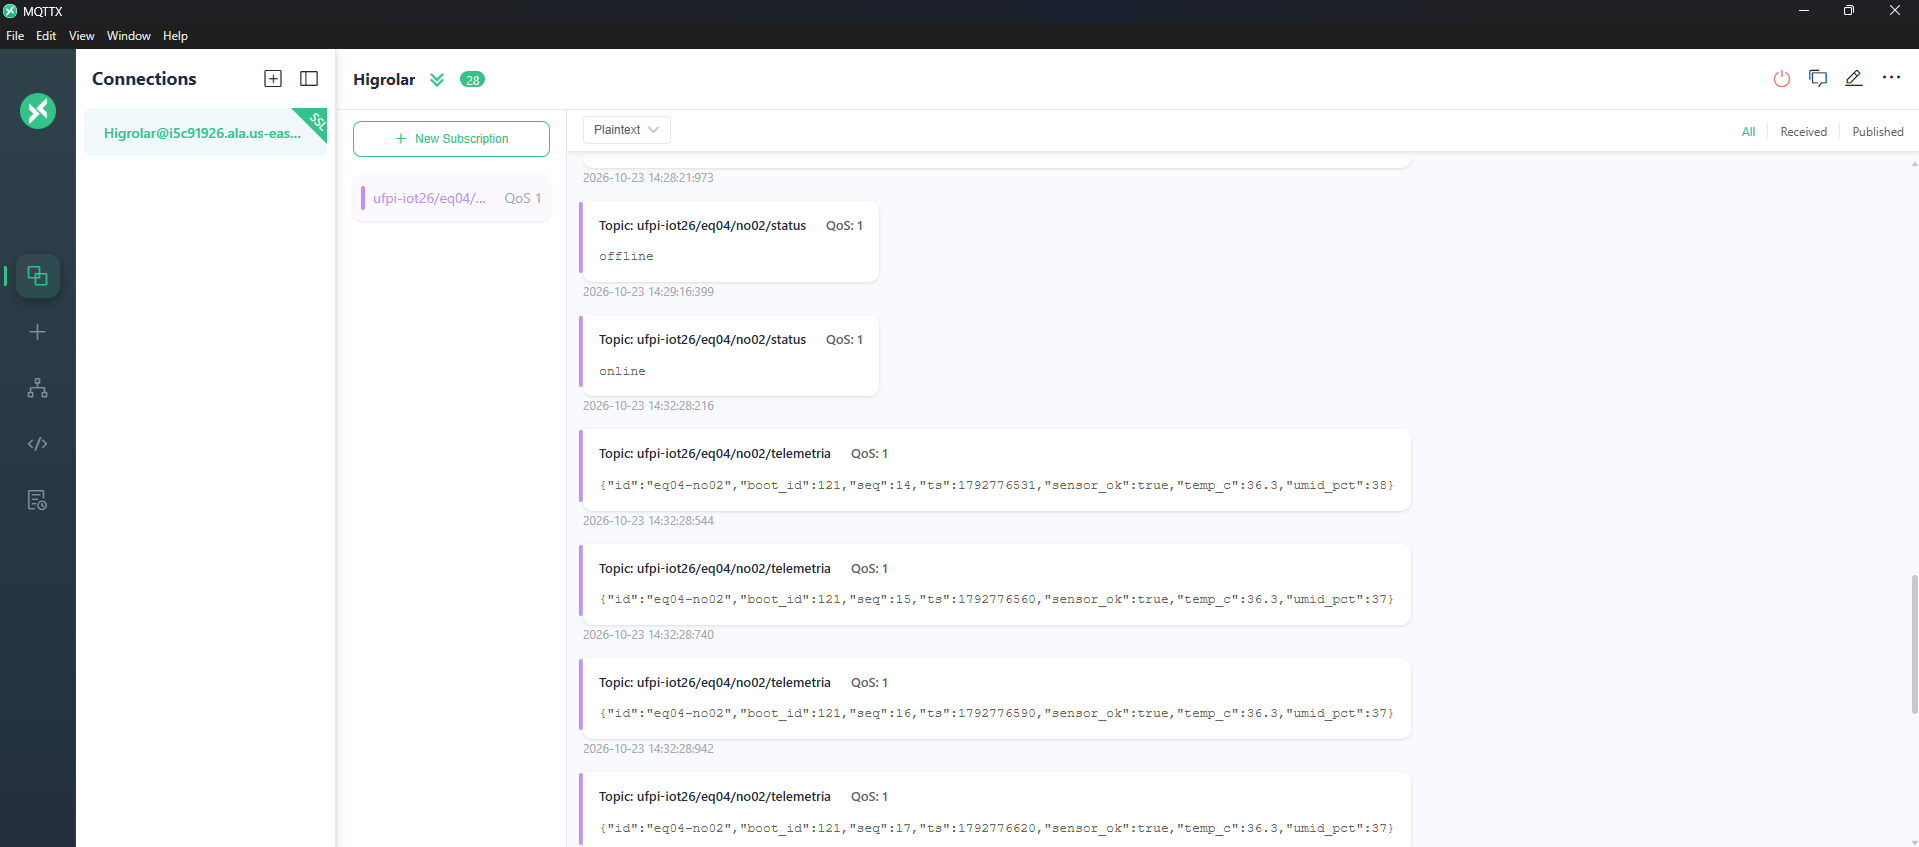
\includegraphics[width=.96\textwidth]{evidencias/prints/mqttx_wifi_retorno.png}\caption{MQTTX evidencia \texttt{offline}, \texttt{online} e retomada da telemetria.}\fonte{Evidência coletada pela equipe em 23/10.}\end{figure}
\begin{figure}[H]\centering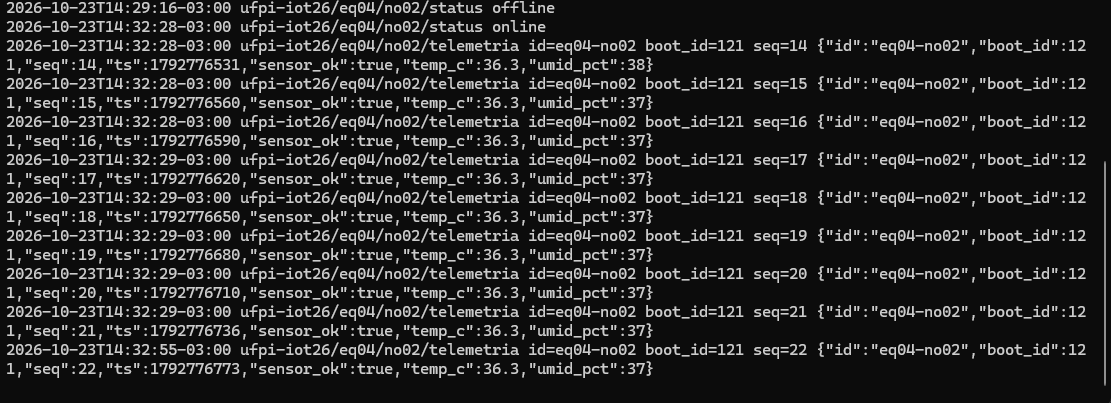
\includegraphics[width=.96\textwidth]{evidencias/prints/gravador_backlog.png}\caption{Console do gravador na recuperação de mensagens acumuladas.}\fonte{PowerShell da coleta eq04.}\end{figure}
\section{Reinício do ESP32, LWT e NTP}
O botão EN foi pressionado às 14h35 de 23/10. O histórico registra \texttt{boot\_id} 121 e depois 122; a sequência recomeça em 1 no novo boot. A primeira mensagem no boot 122 chegou com \texttt{ts:null}; a segunda passou a trazer tempo Unix. Houve eventos de \texttt{offline/online} registrados pelo broker, mas não se cronometrou o intervalo exato entre corte de energia e publicação do testamento. Um estado retido recebido quando o gravador se conecta não deve ser confundido com LWT disparado naquele mesmo instante.
\begin{figure}[H]\centering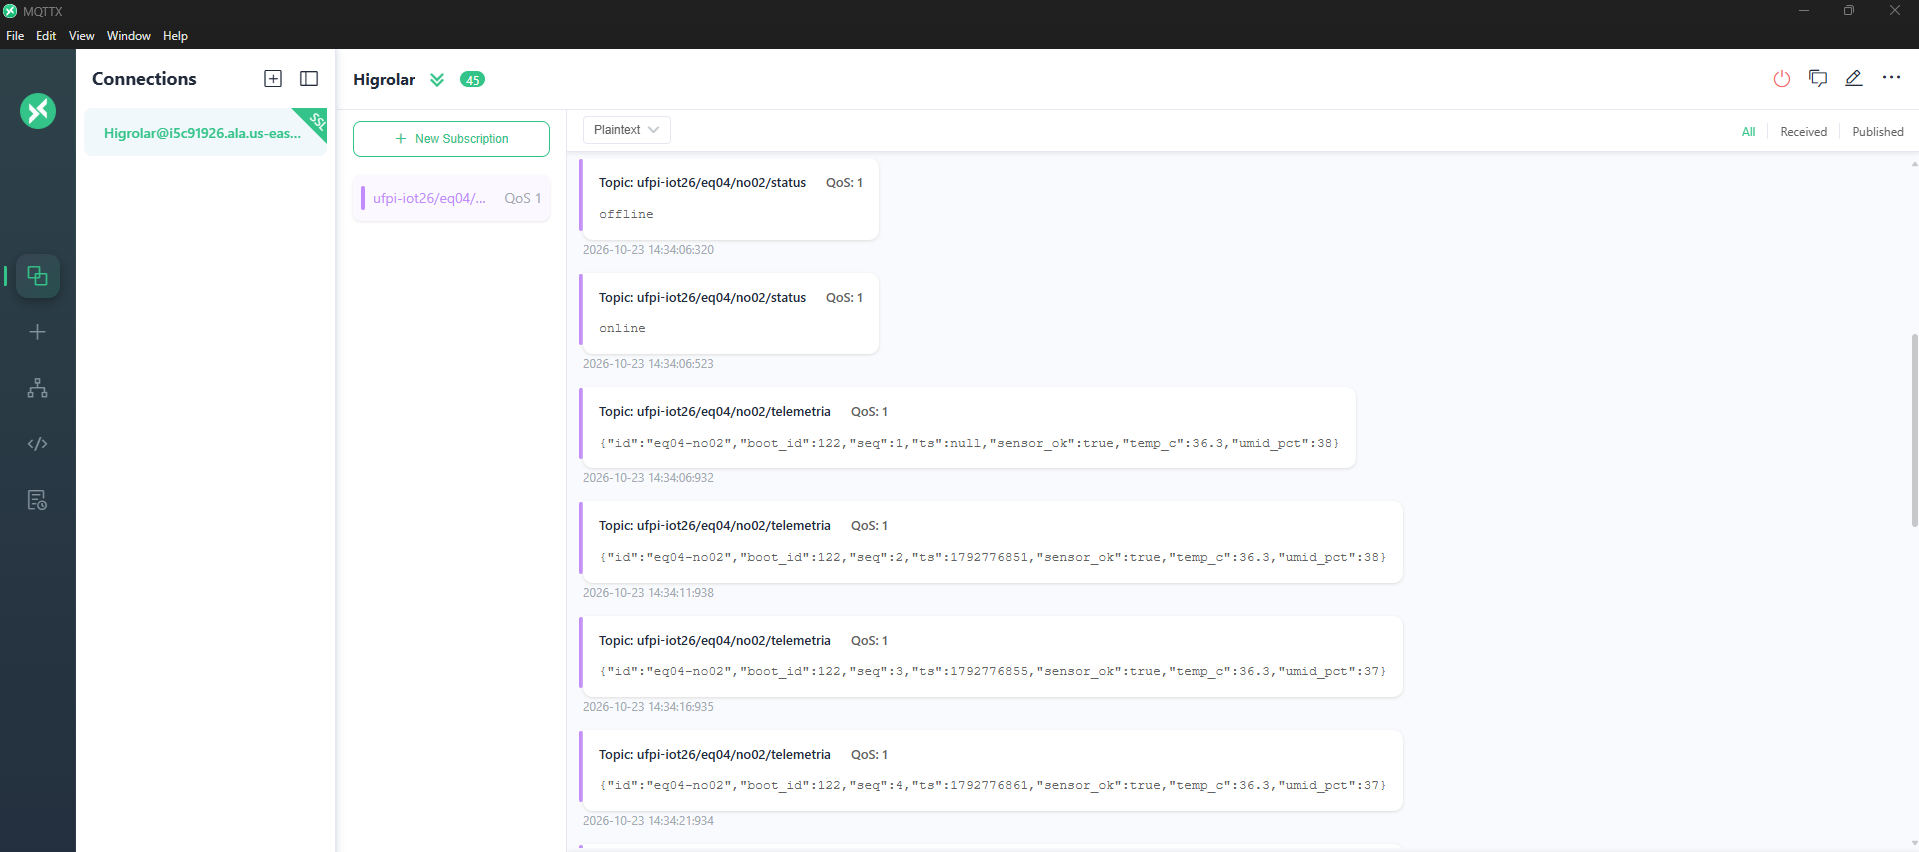
\includegraphics[width=.96\textwidth]{evidencias/prints/mqttx_ntp.png}\caption{Novo \texttt{boot\_id}, sequência reiniciada e primeira leitura antes do sincronismo NTP.}\fonte{MQTTX, 23/10 às 14h34.}\end{figure}
\section{Persistência do gravador e qualidade}
Às 14h38 foi reiniciado o processo de gravação. A conexão subsequente informou sessão anterior existente, com entregas em lote, retomando o CSV com novos registros. O \texttt{qualidade.py} conta duas duplicações lógicas no arquivo final, cuja chave é \texttt{(id,boot\_id,seq)}, mesmo com \texttt{DUP=0}; essa distinção é esperada em QoS 1 e comprova a necessidade de deduplicação \emph{depois} da captura do dado bruto. Um evento extra de \texttt{offline/online} ocorreu em 24/10 às 11h47, mas sua causa não foi identificada no diário; não se atribui artificialmente esse episódio a teste de rede.
\begin{figure}[H]\centering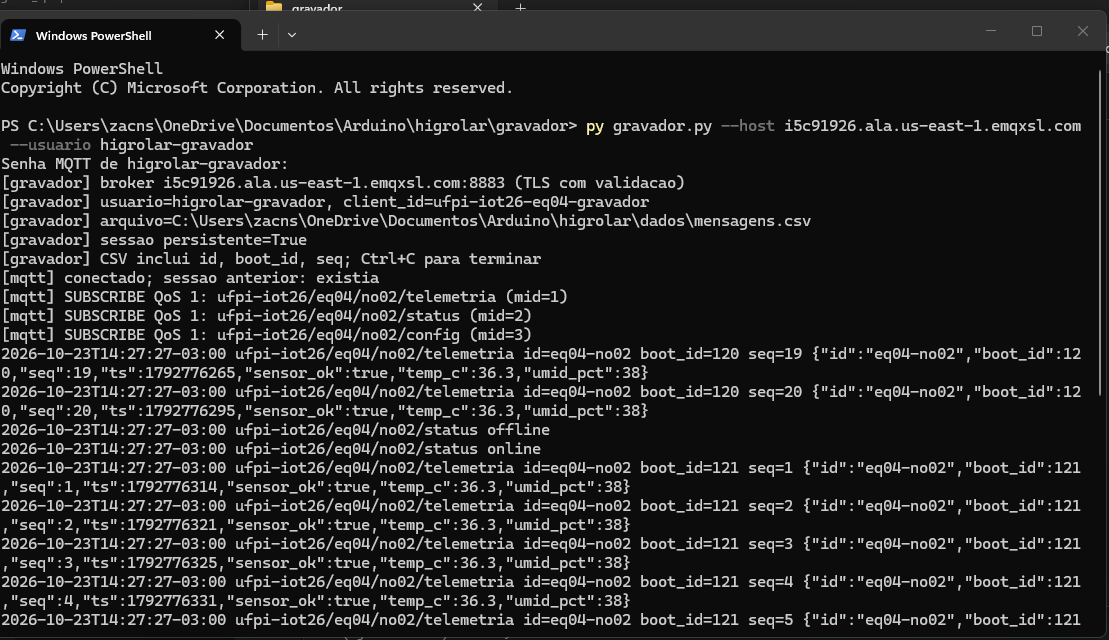
\includegraphics[width=.94\textwidth]{evidencias/prints/gravador_conexao.png}\caption{Inicialização do assinante com TLS, Client ID fixo, inscrição QoS 1 e recebimento de mensagens.}\fonte{PowerShell da equipe.}\end{figure}
\section{Resultados negativos, testes incompletos e reprodução}
O equipamento não dispõe de medição de corrente de Wi-Fi, nem foi aferido o intervalo entre o instante físico da queda de alimentação e a publicação do LWT. O TLS do nó usa \texttt{setInsecure()} quando não há CA embarcada; no EMQX o mecanismo de autorização está em blacklist, com comportamento permissivo fora das regras explícitas. Esses fatos reduzem a avaliação de segurança, mas são declarados para permitir reprodução honesta. O hardware não contém relé para controlar os aparelhos ambientais: as intervenções foram manuais e registradas no diário. A saída integral do programa de qualidade está no Apêndice F e o código correspondente em \texttt{gravador/}.
